% Hotkeys:
% F1 quick build, F7 view pdf, F11 Bibtex

\section{Ridge Regression}
\subsection{Introduction}
Ridge regression is a form of regularization. In regularization high values of the weight coefficients $w$ are penalized. If the weights are of high value it is likely that the generated model is overfitted. The penalizing term is added to the cost function of linear regression, which gives the regularized error of general regularization (Bishop 3.29):
 
\begin{equation}
\frac{1}{2} \sum_{n=1}^{N}((t_n - \bm w^T \phi(\bm x_n))^2)
+ \frac{\lambda}{2} \sum_{j=1}^{J} \lvert{w_j}\rvert^q
\label{regularized_error}
\end{equation}

$N$ is the total number of samples, $t_n$ is the target vector, also referred to as $y$, $w$ is the vector of weight coefficients, $\phi(x)$ is the feature map, $x_n$ the samples, $\lambda$ is the regularization coefficient, $J$ is the number of elements of $w$. Setting $q = 2$ gives the quadratic regularizer ridge regression, while $q = 1$ gives the LASSO estimator.

Again, the feature map $\phi(x)$ is given by a simple polynomial basis with intercept term as in~\cref{eq:polynomial_basis}.

Given the feature map $\phi(x)$ and training set $(x_i, y_i)$ we want to find the coefficient $w$ which minimizes the regularized error~\cref{regularized_error}. To do so, we compute the gradient of the regularized error, set it to zero and solve for $w$. For the quadratic regularizor, there is the following closed-form solution existing (Bishop 3.28):
\begin{equation}
\bm w = (\lambda\bm I + \bm\phi^T\bm\phi)^{-1} \bm \phi^T \bm t 
\label{eq:weights_quad}
\end{equation}

\subsection{Training and testing on the same data}
In this section a model is generated from a given training set and tested on the same dataset. After having determined the weights through ~\cref{eq:weights_quad}, we apply the weights to determine the hyperparameters $\lambda$ and $M$. Fig. \ref{varying_lambda} shows that linear regression ($\lambda$ close to zero) and ridge regression with a low $\lambda$ visually fits the dataset well. This is the case for less complex models with lower degree polynomials. Once the model complexity increases (i.e. $M$ increases) linear regression tends to overfit the data. However, ridge regression is used to restrict the overfitting in complex models. 
This does not seem important in the given example, where the dataset is only two-dimensional. However, higher-dimensional data often requires more complex models to be estimated and therefore often require the use of a regularizor. In Fig. \ref{ridge_him_dim} we can see how linear regression overfits the dataset for a high order polynomial, while ridge regression does not. Fig. \ref{weights_separation} illustrates how a decreasing $\lambda$ separates the weights and an increasing $\lambda$ draws the weights towards zero, also known as \textit{weight decay}.  

\begin{figure}[!ht]
   \centering
   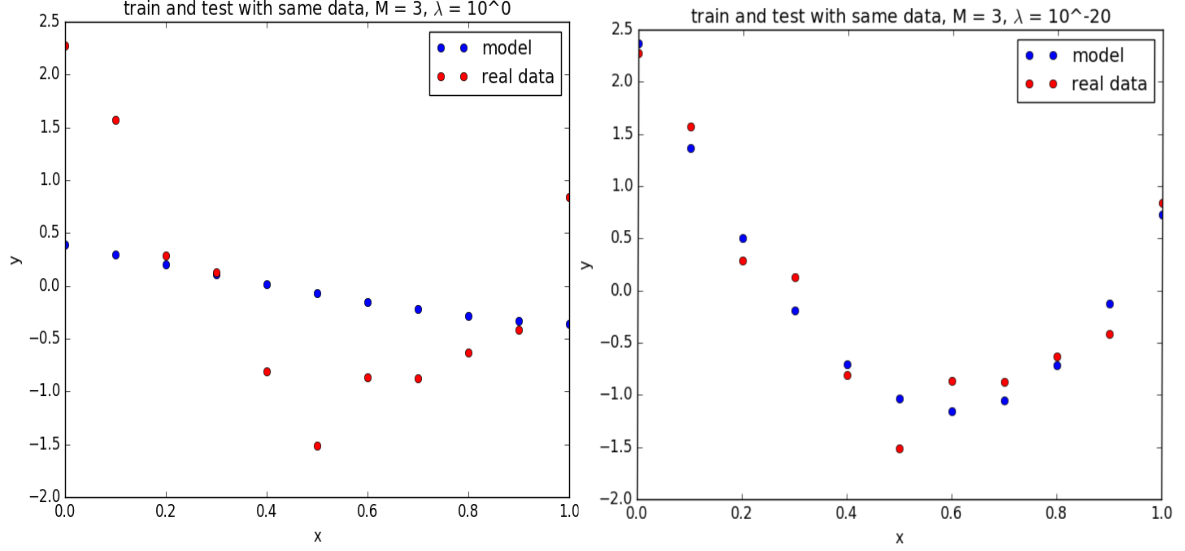
\includegraphics[width=0.9\linewidth]{figures/varying_lambda}
   \caption{The two plots show the effect of a decreasing regularization coefficient $\lambda$ on the estimator. In the left image, the regularization coefficient $\lambda = 1$. If $\lambda$ increases, it penalizes higher weights $w$ stronger, which encourages them to drive to zero. This drives the model target vector $y$ to converge to zero as well (see left). A smaller $\lambda$ does penalize higher weights less, leaving them free to form the polynomial seen on the right. A $\lambda = 0$ would equal an estimator without regularization.}
\label{varying_lambda}
\end{figure}

\begin{figure}[!ht]
   \centering
   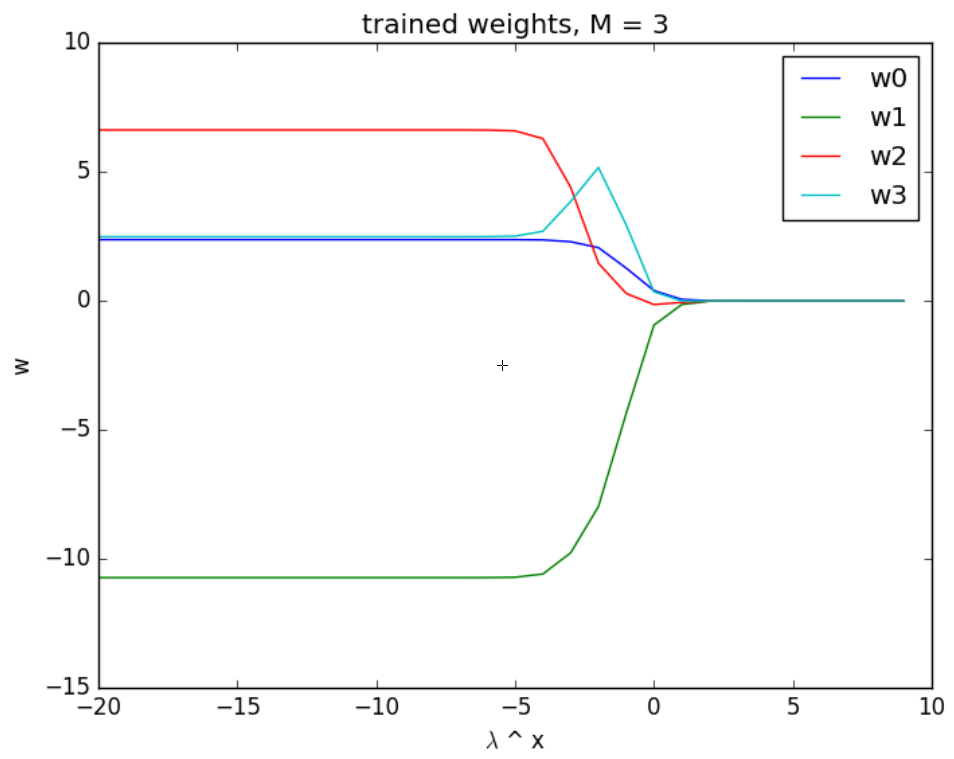
\includegraphics[width=0.8\linewidth]{figures/weights_separation}
   \caption{[x-axis is $log(\lambda)$] If $\lambda$ gets close to zero, the weight coefficients get separated (left). A $\lambda$ of exactly zero would equal the case of not having a regularization term as higher weights $w$ would not get penalized anymore. There is an intersection region around $\lambda=10^{-3}$. After the intersection region $\lambda$ becomes large and drives the weights to zero. There are $M+1$ elements of $w$ (polynomial basis with intercept).}
\label{weights_separation}
\end{figure}

\begin{figure}[!ht]
   \centering
   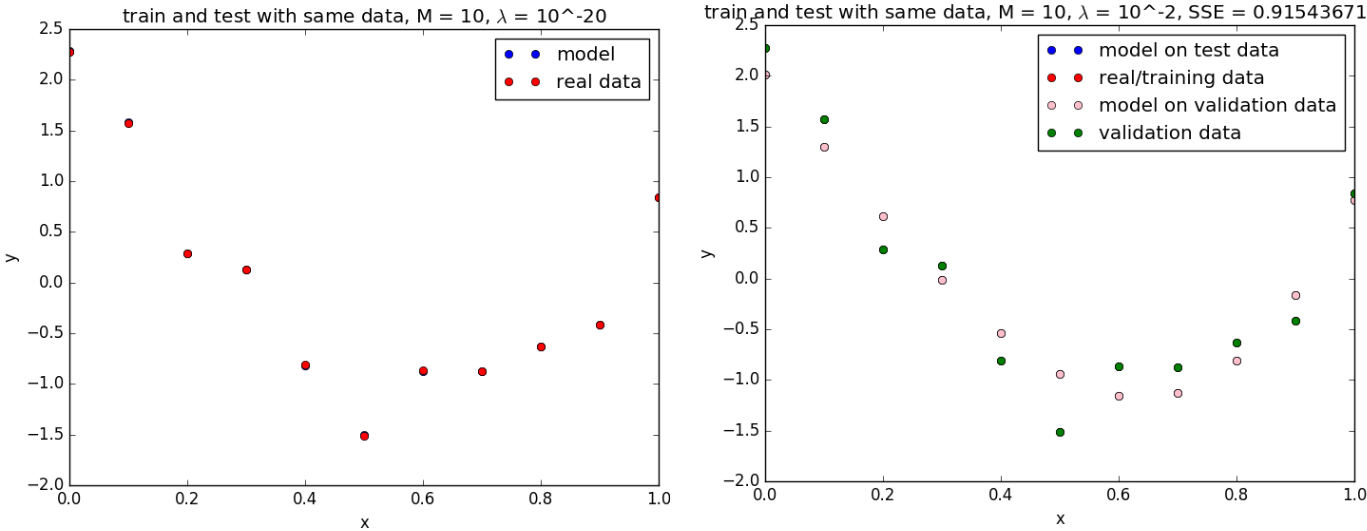
\includegraphics[width=0.9\linewidth]{figures/ridge_high_dim}
   \caption{This plot shows how complex models, represented by a the polynomial feature map $\phi$ of order $M=10$ overfit the data with linear regression (left, where $\lambda \approx 0$). The quadratic regularizor penalizes the high weights and thereby achives to estimate the training data well (right, $SEE \approx 0.92$). Fig. \ref{varying_lambda} in comparison, shows a cubic polynomial feature map. Both, linear and ridge regression have performed comparibly well on low-order models.}
\label{ridge_him_dim}
\end{figure}

\subsection{Training and testing on different data}
In practice, the weights of an estimator are trained on a training dataset, the hyperparameters are determined by a validation data and finally the performance is evaluated on the test dataset. In the earlier section, we have used one dataset for all. Now, we are given  three datasets: A, B and a validation set. Fig. \ref{trainABBA} shows the learned models and their evaluation.

\begin{figure}[!ht]
   \centering
   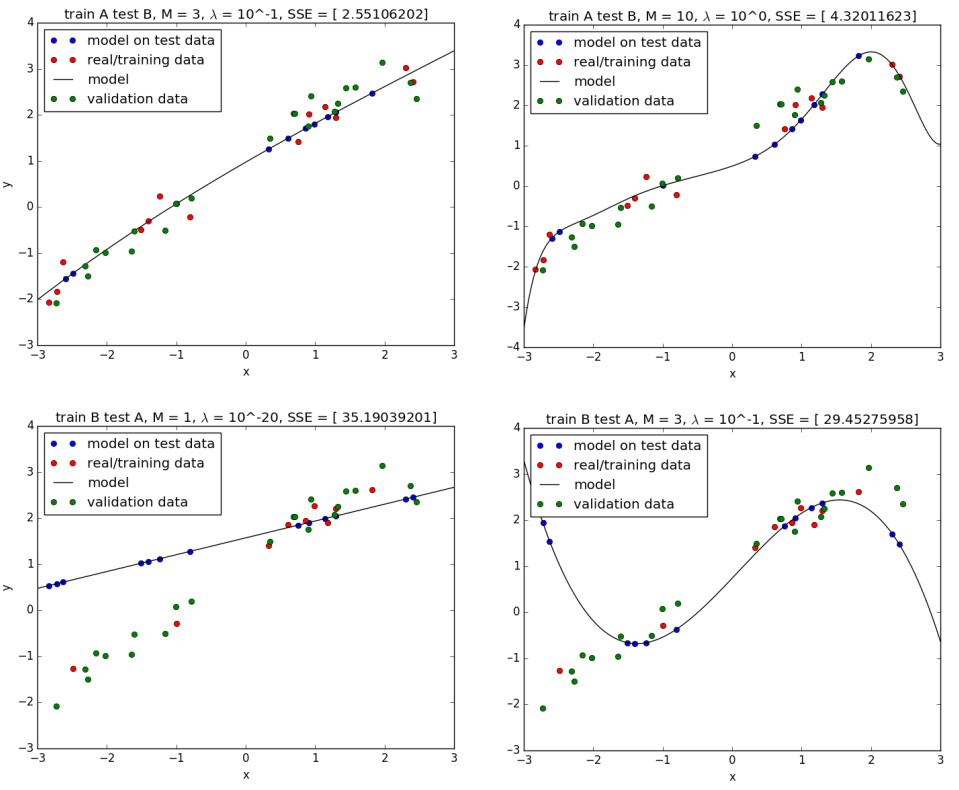
\includegraphics[width=1\linewidth]{figures/trainABBA}
   \caption{The top two figures have trained a model with dataset A, applied on the test data B and the validation dataset. The model has been tested with lower (top-left) and higher (top-right) order polynomials. The higher order one is overfitted although there we have chosen a high value for $\lambda$. Other combinations of $\lambda$ and $M$ have been evaluated according to their $SEE$. The model of degree $M=3$ and $\lambda = 0.1$ has shown the best performance with $SSE = 2.55$ and a visual graphical fit. The dataset B is characterized by one outlier value $(-2.6,3.5)$ (s. bottom plots). In the bottom plots, the model was trained with dataset B and applied to dataset A and the validation data. We can see that the outlier value has significant influence on the learned model and skews the model. We have achieved best fit ($SSE \approx 29.45$) with $M=3$ and $\lambda = 0.1$ (bottom-right). At the same time linear regression performed reasonably well with a linear curve (bottom-left). A solution to use B for training would be preprocessing the data to eliminate outlier values.}
\label{trainABBA}
\end{figure}

The sum of least squares error (SSE) is a valuable measurement index to evaluate the performance of a trained model. The SSE is given by ~\cref{eq:sse}. Varying along the hyperparameters we can find the one with the best fit on the validation data. Table \ref{table_sse} shows the influence of a varying regularization coefficient $\lambda$. For training with A, a $\lambda$ around zero shows the best results, while a training with B has the best performance with $\lambda = 1$. Further evaluation of the model can be achieved by looking at the R squared error, which will produce similar results in a scale adapted the mean of the validation dataset. 

\begin{table}[ht!]
\centering
\begin{tabular}{||c c c||}  
 \hline
 $log(\lambda)$ & $SSE_A$ & $SSE_B$ \\ [0.5ex] 
 \hline\hline
 -20 & 2.37 & 35.19 \\ 
 \hline
 -1 & 2.55 & 34.80 \\
 \hline
 0 & 4.35 & 32.10 \\
 \hline
 1 & 16.17 & 32.18 \\
 \hline
 2 & 29.54 & 62.68 \\
 \hline
 10 & 76.51 & 76.51 \\ [1ex] 
 \hline
\end{tabular}
\caption{Effect on $\lambda$ on the sum of least squares error $SSE$ on model trained with A and B and compared to validation dataset. A polynomial of $M=3$ and $M=1$ has been used for training with A and B, respectively.}
\label{table_sse}
\end{table}

\section{Sparsity and Lasso}
In ridge regression we have used a quadratic regularizor, which corresponds to the general regularized error function \ref{regularized_error}, where $q = 2$. Least absolute shrinkage and selection operator (Lasso) uses the $L_1$ norm, $q = 1$ to compute the error. Lasso gives a sparse solution model, i.e. by increasing the $\lambda$, it drives some weight coefficients to exactly zero. In this chapter, we compare the performance of Lasso to ridge regression. 

A newly given dataset was generated by a sinoid feature vector and small noise $\epsilon$. The feature vector is given by:

\begin{equation}
\phi(x) = (x, sin(0.4\pi * 1),..., sin(0.4\pi x * 12)) \in{\rm I\!R}^{13}
\label{lasso_feature}
\end{equation}

In Fig. \ref{lasso_lambda}, we can see that $\lambda = 0.1$ leads to a sparse estimation of the weight vector $w$ and only four values remain non-zero. Visualized in 2D, Lasso drives a weight tuple into the corners of a rectangle. Ridge regression drives the weights onto the circumference of a circle (Bishop 3.1.4).

\begin{figure}[!ht]
   \centering
   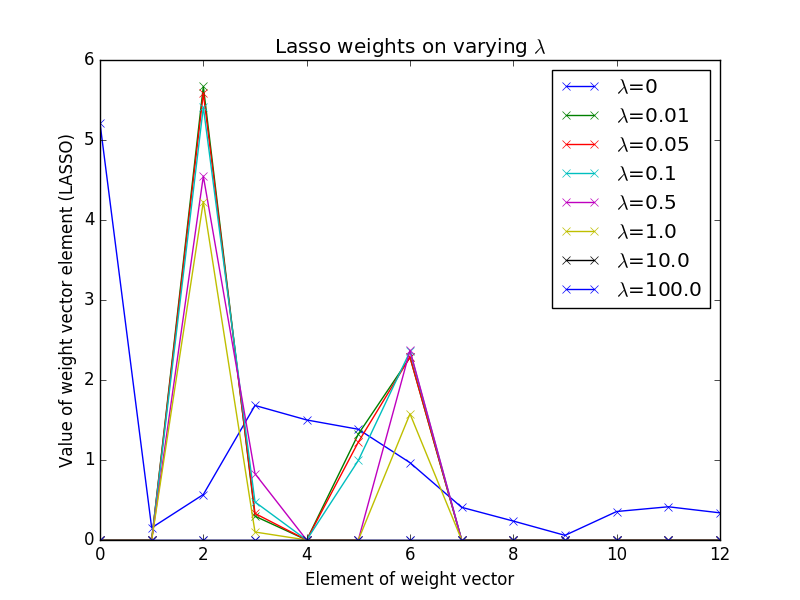
\includegraphics[width=0.9\linewidth]{figures/lasso_lambda}
   \caption{This graphs shows the relation the lasso regularization coefficient $\lambda$ to the weight vector $w$. $\lambda = 0$ equals an estimator without regularizing term. The further the $\lambda$ increases, the further the weight elements are decaying to zero. $\lambda = 0.01$ leads to a reasonable separation of the weight vector, where four elements are non-zero: $w_2, w_3, w_5$ and $w_6$}
\label{lasso_lambda}
\end{figure}

We compare the weight coefficient from Lasso with the weights from ridge and the true $w$ in Fig. \ref{lasso_weights} and visual inspection shows us that the estimated weights by lasso are very close to the true weights.

\begin{figure}[!ht]
   \centering
   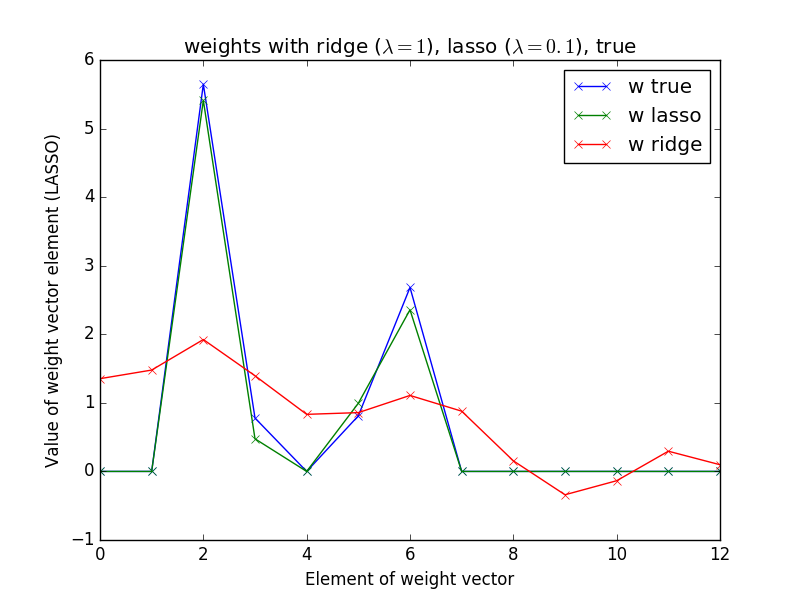
\includegraphics[width=0.9\linewidth]{figures/lasso_weights}
   \caption{This figure displays the weights from the lasso regularizor ($\lambda = 0.1$) with the estimated weights from ridge ($\lambda = 1$) and the true ones. On visual inspection, the lasso weights are very close to the true weights. All elements of the lasso weight vector have decayed to zero, such that only four non-zero elements remain. The weights from ridge regression differ strongly from the true weights and no weights are zero.}
\label{lasso_weights}
\end{figure}

In~\cref{regularizor_comparison}, we use the learned weights of ridge, lasso and the true ones onto our validation dataset. This gives us knowledge about the fit of the estimator on the real data.
Based on the smooth plot in~\cref{regularizor_comparison} and the low SSE in~\cref{table:sse_weights}, Lasso seems to generate the best model of this dataset. 
 
\begin{table}[ht!]
\centering
\begin{tabular}{||c c c c||}  
 \hline
 \ & $SSE_{val}$ & $SSE_{test}$ & $SSE_{train}$ \\ [0.5ex] 
 \hline\hline
 Lasso & 1.13 & 1.39 & 0.19 \\ 
 \hline
 Ridge & 4.03 & 7.50 & 1.70 \\
 \hline
 True & 0.41 & 0.39 & 0.25 \\[1ex] 
 \hline
\end{tabular}
\caption{This tables compares the estimators according to their sum of least squares error. We see that Lasso performs better than ridge on the validation and teh test dataset. I would not be useful to select an estimator by only looking on its performance on the trained data, as an overfitted model could achieve an error $SSE_{train}=0$. In comparison to the true data, we see that Lasso performs reasonably well.}
\label{table:sse_weights}
\end{table}

\begin{figure}[!ht]
   \centering
   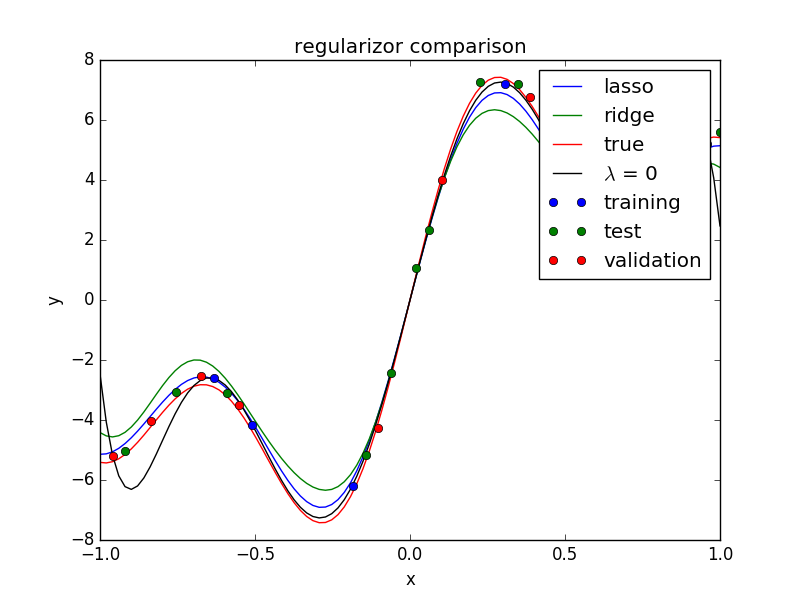
\includegraphics[width=0.9\linewidth]{figures/regularizor_comparison}
   \caption{In the plot, we have compared the performance the learned models from Lasso, ridge and linear regression ($\lambda = 0$) with the true sinoid function. The used weights are the ones displayed in~\cref{lasso_weights}. The plot also shows the used training, test and validation datasets. We can observe, that the model for the true weights and lasso weights is visually very close to the validation and test dataset. This observation gets confirmed by Table~\cref{table:sse_weights}, in which we have analysed the $SSE$ of the estimators. For this data we would select the Lasso estimator for evaluating a test dataset. The datapoints of the validation data do not fit onto the true sinoid curve, because they have been generated by adding small random noise.}
\label{regularizor_comparison}
\end{figure}


\section{Conclusion}
We have given provided a look into gradient descent, linear basis function regression, ridge regression, sparsity and LASSO. Different datasets, weights and hyperparameters have been tested and compared regarding their performance.